\section{Typical Impedance Measurement Principles} \label{sec:TypicalMeasPrin}
Throughout the time numerous different methologies have been utilized to measure impedance. Historically the AC Wienbridge circuits has been generously used in the 
early days of electronics, back before even the transistor was a common component \cite{IET_LABS_LCR_PRINCIPLES}. As demands for the electronics industry grew tighter,
faster and more accurate methods were developed, such as the auto balancing bridge circuit, using negative feedback to amplify the current, allowing for even the
smalles amount of current to be measured.

This section will describe some of the most common methods used through the time to measure impedance, these are the bridge topology, the auto balancing bridge, and a more advanced
and complicated version of the auto balancing bridge. 

\subsection{Wheatstone Bridge}
The Wheatstone bridge has been around since then 
\begin{figure}[H]
    \centering
    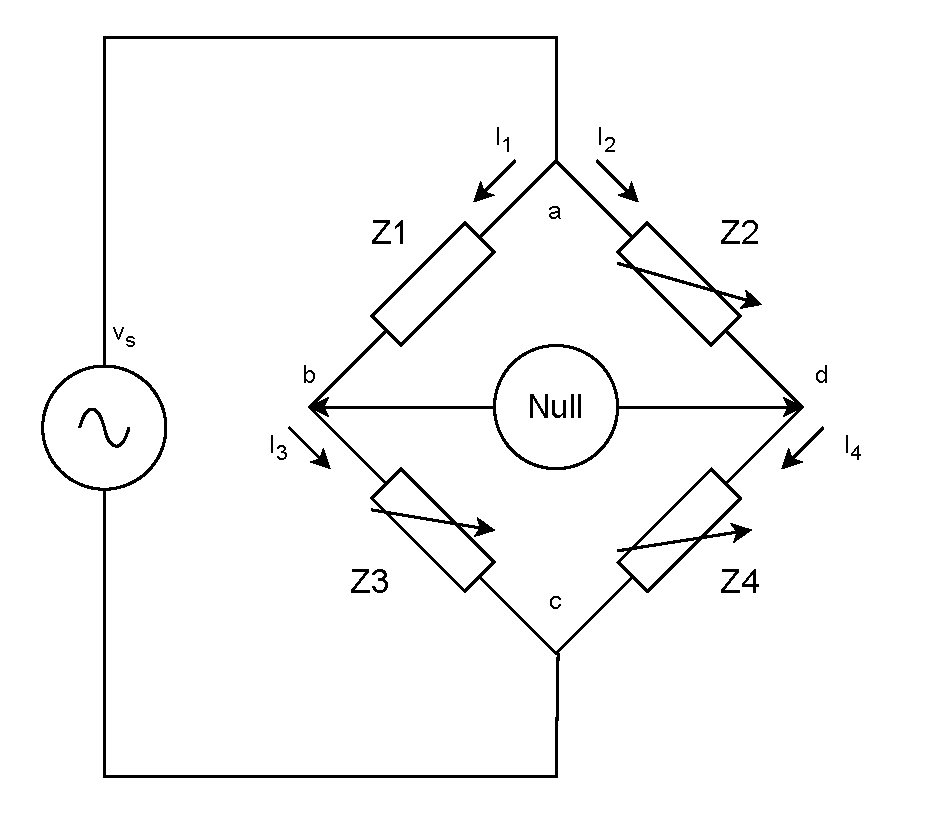
\includegraphics[width=1\textwidth]{Sections/4_TechnicalAnalysis/Figures_JFT/WheatstoneBridgeAC.pdf}
    \caption{A typical AC Wheatstone bridge, where Z1 is the device under test.}
    \label{fig_4_2_WheatstoneBridge}
\end{figure}